\documentclass[11pt,a4paper]{article}
\usepackage[utf8]{inputenc}
\usepackage{amsmath}
\usepackage{amsfonts}
\usepackage{amssymb}
\usepackage{graphicx}
\usepackage{booktabs}
\usepackage{multirow}
\usepackage{subcaption}
\usepackage{microtype}
\usepackage[left=2cm,right=2cm,top=2cm,bottom=2cm]{geometry}
\author{Yi Hao}
\title{Training Dynamics of Heavy-Tailed Initialisation in Deep Learning}
\begin{document}
\maketitle
\section{Abstract}
Conventional deep learning theory typically assumes Gaussian weight statistics, leading to narrow critical points that necessitate precise parameter fine-tuning. In contrast, recent analytical frameworks suggest that heavy-tailed initializations ($\alpha < 2$) enable the emergence of an extended critical regime. This regime provides significant computational advantages by balancing the contraction and expansion of internal neural representations across the network depth. This study investigates the non-equilibrium weight trajectories of a 10-layer MLP initialized at $\alpha = 1.2$ to identify the dynamical mechanisms underlying these advantages. Our preliminary observations reveal a profound spatial decoupling of learning dynamics: early hidden layers exhibit high-energy, symmetric displacement consistent with a diffusive stochastic reservoir, while terminal layers display sparse, high-magnitude upward spikes in displacement. We speculate that these terminal layers are in a directed ballistic state, where their movements are highly correlated with one another but functionally decoupled from the shallower layers. This hierarchical division of labour suggests that while early layers provide a stable foundation for signal propagation, the deep layers leverage extended criticality to perform the discrete, directed structural realignments, or Lévy flights that drive observed staircase improvements in classification performance.
\section{Introduction}
\section{Related Works}
\section{Method}
\subsection{Heavy-Tailed Initialization and Extended Criticality}

To investigate the non-equilibrium dynamics of deep neural networks (DNNs) beyond the Gaussian regime, we initialize the weight matrices $W^l$ using symmetric $\alpha$-stable distributions, as defined by the characteristic function:
\begin{equation} \label{eq:levy_alpha}
    \varphi(u; \alpha, \beta, \sigma, \mu) = \exp\left(-|\sigma u|^\alpha (1 - i\beta \text{sgn}(u)\Phi(u; \alpha)) + iu\mu\right)
\end{equation}
Following the framework of Lévy mean-field theory, we assume a symmetric distribution where the skewness $\beta$ and location $\mu$ are set to zero. The stability parameter (tail index) is set to $\alpha < 2.0$, placing the network within the analytically predicted extended critical regime.

\subsubsection{Scaling Laws and Effective Layer Size}
To ensure consistent signal propagation and avoid the vanishing or exploding gradient problems associated with deep architectures, we adopt a scaling law for the weight entries $W_{ij}^l \sim S_\alpha((D_w / 2N)^{1/\alpha})$. In our implementation, we define an effective width $N_{\text{eff}}$ to normalize the scale parameter across varying layer geometries:
\begin{equation}
    N_{\text{eff}} = 
    \begin{cases} 
      \sqrt{N_{in} \cdot N_{out}} & \text{for linear layers} \\
      C_{in} \cdot K_h \cdot K_w & \text{for convolutional layers}
    \end{cases}
\end{equation}
The scale parameter $\sigma$ for the stable distribution is then computed as:
\begin{equation}
    \sigma = \frac{g}{(2 N_{\text{eff}})^{1/\alpha}}
\end{equation}
where $g$ represents the global gain factor (equivalent to $D_w^{1/\alpha}$ in the manuscript). This normalization ensures that the fluctuations of the neural input distribution remain stable across the depth of the network. The classical setup is recovered in the $\alpha \rightarrow 2$ limit for comparison with standard Gaussian dynamics.

\subsubsection{Stochastic Implementation}
Weight initialization is performed using a localized pseudo-random number generator for each layer $l$:
\begin{equation}
    W^l \leftarrow \text{Lévy\_Stable}(\alpha, \beta=0, \sigma, \text{seed} = S_{base} + l)
\end{equation}
By decoupling the random seeds across layers, we prevent the formation of correlated super-paths of outliers through the network depth. This ensures that the observed multifractal properties of the layerwise Jacobians are a result of the collective heavy-tailed dynamics rather than initialization artifacts.

\subsection{Dynamical Observables: Layer-wise Displacement Tracking}

To quantify the evolution of the network weight manifold during training, we define three primary scalar observables derived from the weight displacement vector. Let $W^l_t$ denote the weight matrix of layer $l$ at training step $t$. For a specific time lag $\tau$, the displacement matrix is defined as $\Delta W^l(t, \tau) = W^l_t - W^l_{t-\tau}$. These metrics allow us to distinguish between stochastic noise, collective drift, and high-energy structural realignments.

\subsubsection{Mean Net Displacement (Drift)}
The Mean Net Displacement, $\mu_{\Delta W}$, represents the collective drift or center-of-mass movement of the parameters in layer $l$:
\begin{equation}
    \mu_{\Delta W}(t, \tau) = \frac{1}{N_l} \sum_{i,j} \Delta W^l_{ij}(t, \tau)
\end{equation}
where $N_l$ is the total parameter count for the layer. This observable serves as a dynamical indicator of symmetry breaking; values fluctuating near zero suggest a state of local stochastic equilibrium, whereas sustained plateaus signify a directed migration toward a new representation.

\subsubsection{Mean Absolute Displacement (L1 Activity)}
The Mean Absolute Displacement provides a measure of the total integrated activity of the layer, independent of direction:
\begin{equation}
    \mu_{|\Delta W|}(t, \tau) = \frac{1}{N_l} \sum_{i,j} |\Delta W^l_{ij}(t, \tau)|
\end{equation}
This $L_1$ metric captures the typical scale of weight updates. It is used to identify the thermal floor of the training process and detect changes in the overall volume of weight exploration across different network depths.

\subsubsection{Root Mean Square Displacement (L2 Energy)}
The Root Mean Square (RMS) displacement, or $L_2$ norm, characterizes the total kinetic energy of the layer-wise updates:
\begin{equation}
    \text{RMS}_{\Delta W}(t, \tau) = \sqrt{\frac{1}{N_l} \sum_{i,j} \left( \Delta W^l_{ij}(t, \tau) \right)^2}
\end{equation}
By squaring the displacements before averaging, the $L_2$ norm is significantly more sensitive to outliers than the $L_1$ norm. In networks initialized with heavy-tailed distributions ($\alpha < 2$), this observable is the primary detector for Lévy flights, discrete, high-magnitude realignments that dominate the transport physics in the extended critical regime.

\subsubsection{Multi-Scale Temporal Analysis}
To separate microscopic noise from macroscopic learning, these metrics are tracked across two distinct time lag regimes:
\begin{enumerate}
    \item \textbf{Microscopic Lag ($\tau < 1$ epoch):} Captures the instantaneous stochastic gradient noise and the thermal floor of the initialization.
    \item \textbf{Macroscopic Lag ($\tau \geq 1$ epoch):} Acts as a low-pass filter to reveal persistent structural drift and global phase transitions that are otherwise obscured by step-wise jitter.
\end{enumerate}

All macroscopic lag data points are timestamped at the window midpoint, $t - \tau/2$, to ensure causal alignment between internal weight reorganization and external performance metrics such as test accuracy and loss.
\section{Experiments}
\subsection{Dataset and Preprocessing}
All experiments are conducted using the MNIST dataset of handwritten digits. The input data consists of $28 \times 28$ grayscale images, which are flattened into vectors of size 784. Preprocessing involves a standard normalization transform with a mean of 0.1307 and a standard deviation of 0.3081. We utilize a consistent batch size of 1024 to maintain stable gradient estimates across all initialization regimes.

\subsection{Model Architecture}
To study the impact of heavy-tailed statistics on non-equilibrium learning dynamics, we employ a deep Multilayer Perceptron (MLP) consisting of $L=10$ layers (9 hidden layers and one output classifier). The network maps an input vector $x^0 \in \mathbb{R}^{784}$ to an output $x^L \in \mathbb{R}^{10}$ through a sequence of transformations:
\begin{equation}
    x^l = \phi(W^l x^{l-1} + b^l)
\end{equation}
where $\phi$ is the activation function. The specific architectural constraints are defined as follows:

\begin{itemize}
    \item \textbf{Layer-wise Dimensions:} We maintain a constant hidden width of $N=784$ neurons for all layers $l \in \{1, \dots, L-1\}$. This configuration ensures that the weight matrices $W^l$ are square ($N \times N$), facilitating direct comparisons with results from Random Matrix Theory (RMT) and free probability.
    \item \textbf{Weights ($W$):} The weight matrices $W^l$ are initialized according to a symmetric $\alpha$-stable distribution. This initialization places the network within the extended critical regime, distinct from standard Gaussian ($\alpha=2$) initializations.
    \item \textbf{Activation ($\phi$):} The hyperbolic tangent ($\tanh$) function is utilized for all hidden layers to ensure bounded signal propagation and centred activations.
    \item \textbf{Biases ($b$):} All bias terms are explicitly disabled ($b^l=0$) to isolate the dynamical effects of the weight matrix couplings and simplify the analysis of the layer-wise Jacobians.
\end{itemize}

\subsection{Heavy-Tailed Initialization Strategy}
The core of this research involves a parametric sweep over non-Gaussian weight initializations. Weights are sampled from a symmetric L\'{e}vy $\alpha$-stable distribution defined by Eq. \ref{eq:levy_alpha}. We explore a $3 \times 3$ grid of hyperparameters to compare different dynamical phases:
\begin{itemize}
    \item \textbf{Stability Parameter ($\alpha$):} Fixed at $\{1.2, 1.5, 2.0\}$. Here, $\alpha=2.0$ serves as the Gaussian baseline, while $\alpha < 2.0$ introduces heavy-tails with infinite variance.
    \item \textbf{Scale Parameter ($g$):} Fixed at $\{0.25, 1.0, 3.0\}$. This parameter dictates the coupling strength $D_w^{1/\alpha}$, allowing us to move the network through ordered, critical, and chaotic regimes.
\end{itemize}

\subsection{Optimization and Training Protocol}
The networks are trained for 650 epochs using vanilla Stochastic Gradient Descent (SGD). We set a fixed learning rate of $\eta = 0.001$. Notably, we omit momentum and weight decay; this ensures that any observed structural evolution or rich learning behaviour is a direct result of the interaction between the heavy-tailed initialization and the fundamental SGD trajectory. All simulations are executed on NVIDIA hardware using the PyTorch framework with a fixed seed ($s=0$) to ensure exact reproducibility across parameter sweeps.
\section{Results}
The performance of the 10-layer MLP was evaluated across a $3 \times 3$ grid of initialization parameters, varying the tail index $\alpha \in \{1.2,1.5,2.0\}$ and the scale factor $\sigma \in \{0.25,1.0,3.0\}$. These parameters were selected to represent the ordered, critical, and chaotic regimes, respectively.

\begin{figure}[htbp]
    \centering
    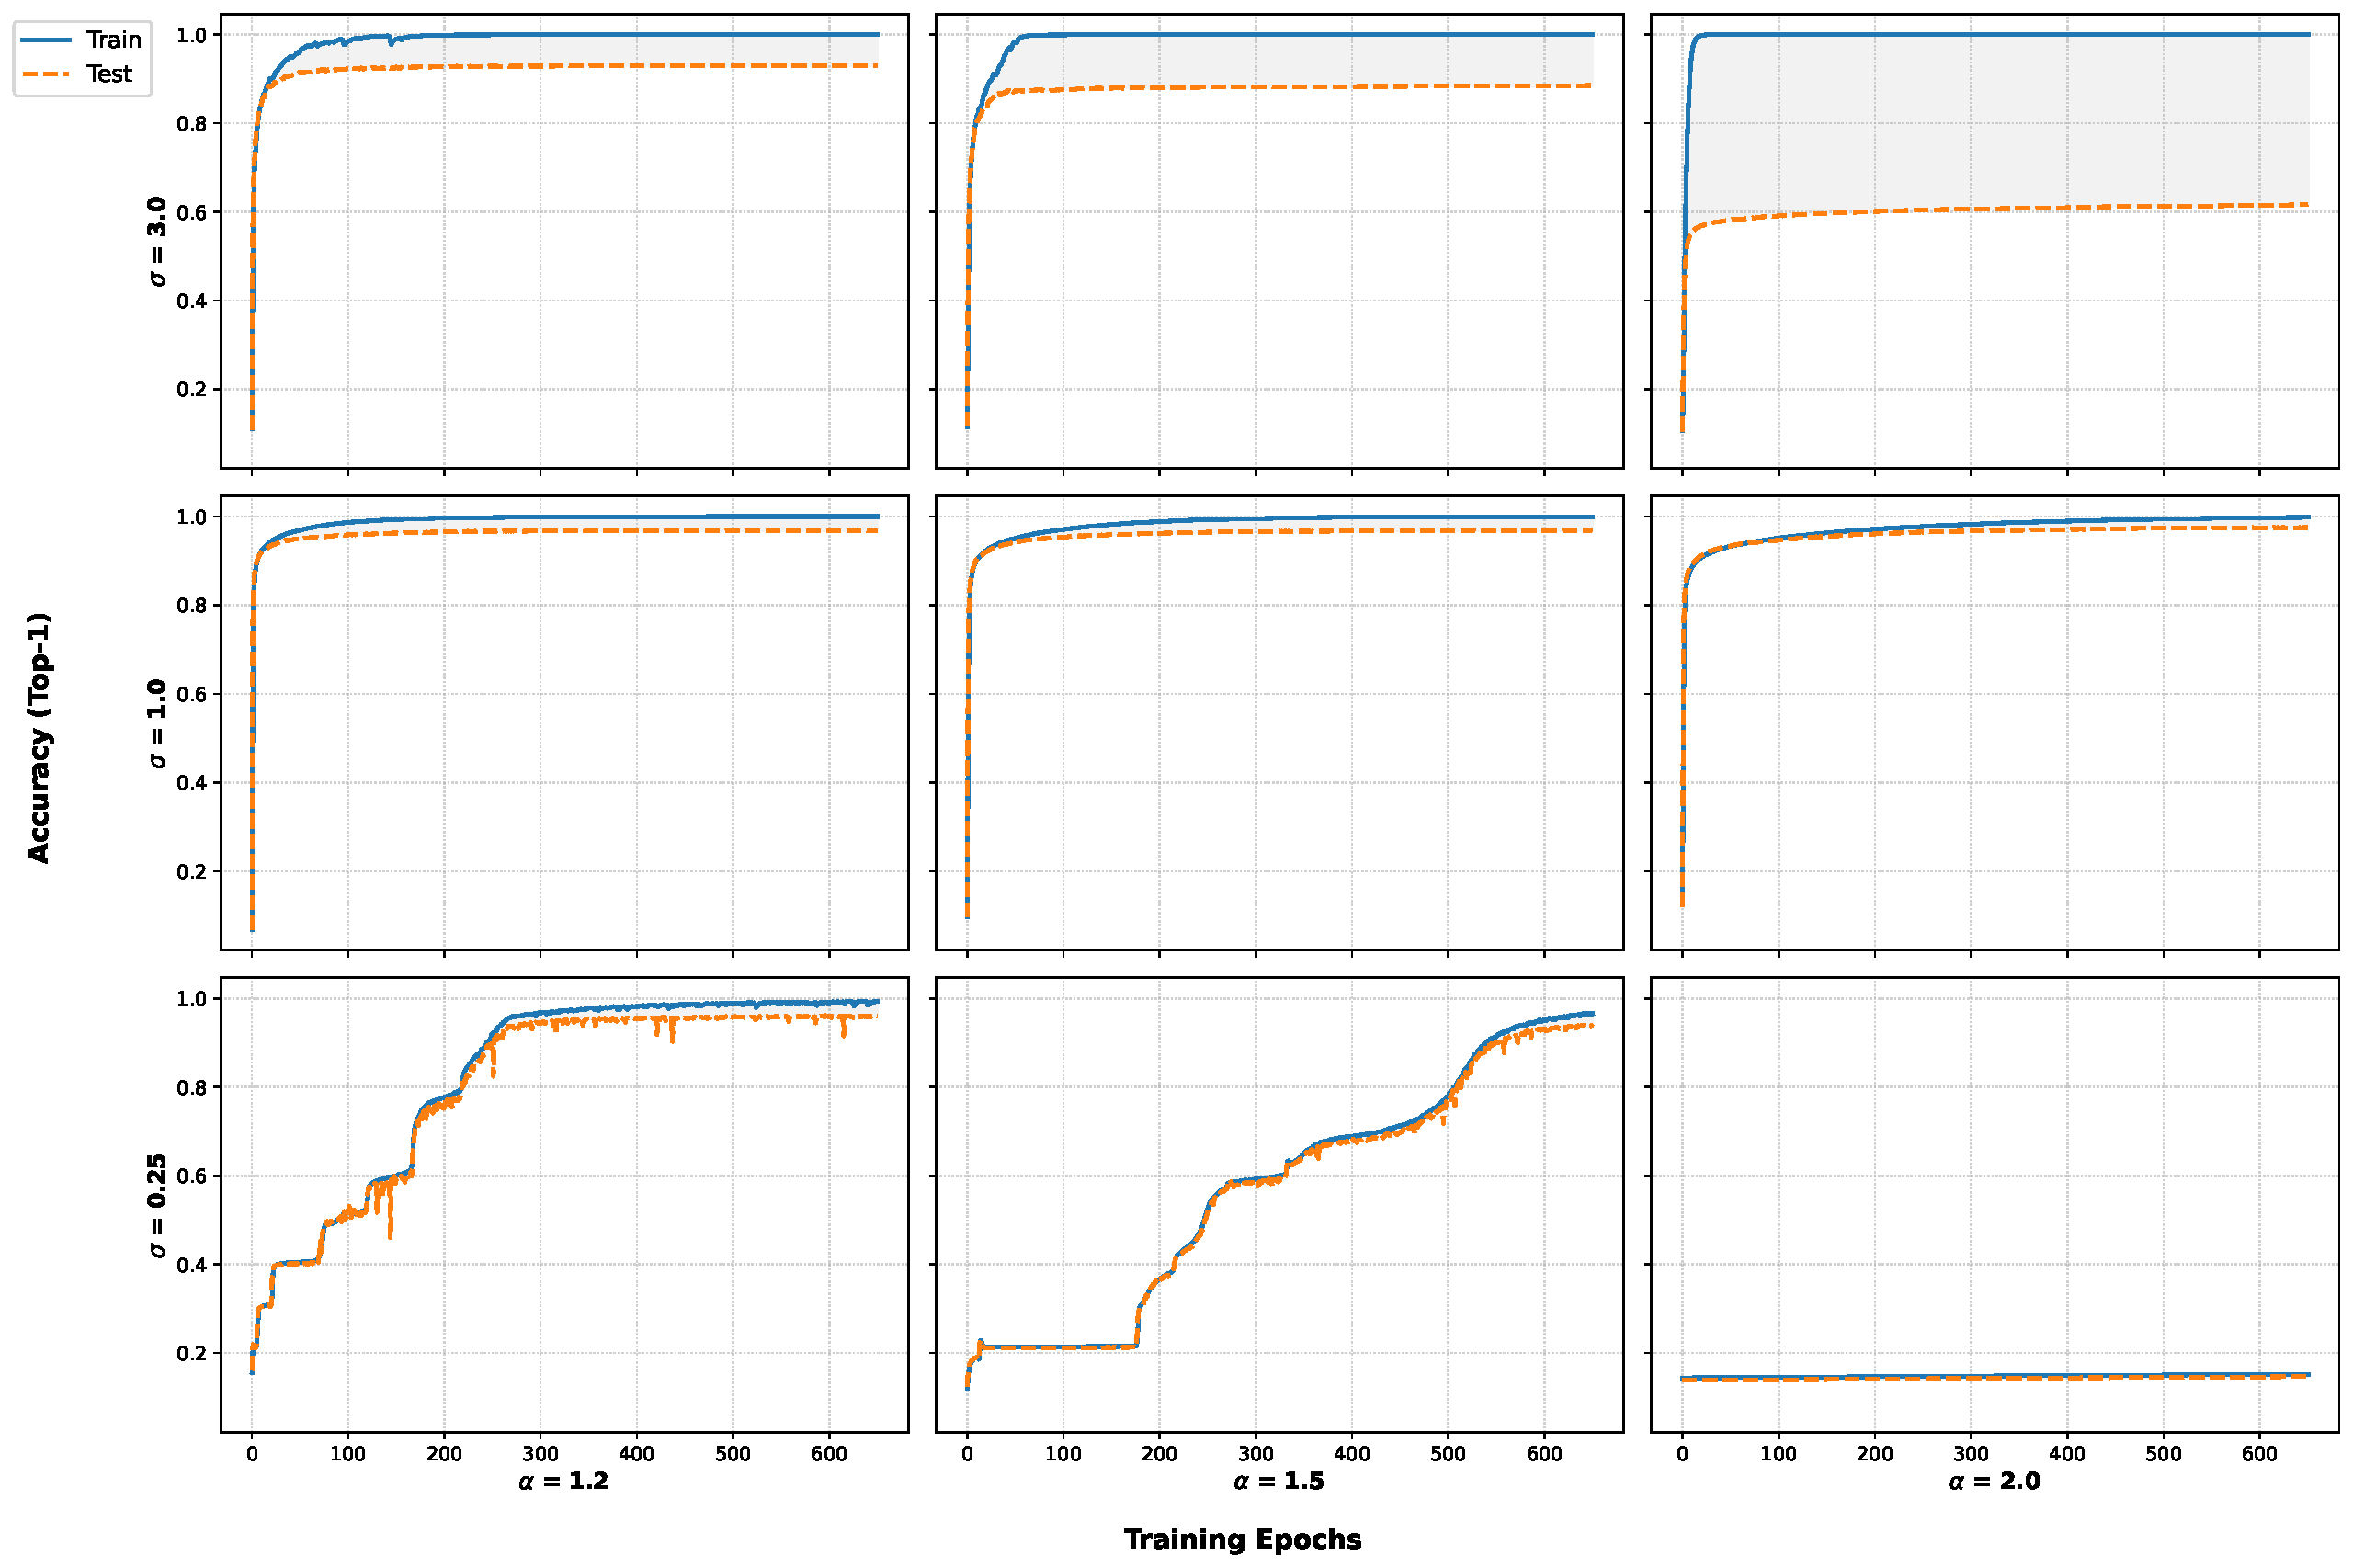
\includegraphics[width=0.8\textwidth]{performance_runs.pdf}
    \caption{Accuracy curves for 10-layer MLP trained on MNIST. Initialisation varies from Gaussian ($\alpha = 2.0$) to strongly heavy-tailed ($\alpha = 1.2$), while the three scale values of $\sigma = 0.25, 1.0, 3.0$ are chosen to represent the ordered, critical, and chaotic regimes respectively. Generalisation gap is highlighted in grey.}
    \label{fig:performance_curves}
\end{figure}

The training profiles across the $3\times3$ parameter sweep, as detailed in Figure \ref{fig:performance_curves} and Table \ref{tab:performance_summary}, exhibit dynamical behaviours consistent with the extended critical regime described in recent theoretical frameworks. 

The training trajectories and final performance metrics, summarized in Table \ref{tab:performance_summary}, reveal distinct behaviours across the parameter space. Within the critical regime ($\sigma=1.0$), all configurations exhibit robust convergence. The Gaussian ($\alpha=2.0$) initialization achieves the highest test accuracy in this regime at 0.9751, followed closely by the heavy-tailed variants. However, as the system moves into the ordered and chaotic regimes, a significant divergence in performance emerges.

In the chaotic regime ($\sigma=3.0$), the Gaussian network suffers from a substantial generalization gap of 0.3836. In contrast, the heavy-tailed configurations ($\alpha=1.2,1.5$) demonstrate superior stability, maintaining test accuracies above 85\%, with the $\alpha=1.2$ run achieving 0.9297. This suggests that heavy-tailed initialization may provide a degree of protection against the informational expansion typically associated with chaotic phases.

\begin{table}[htbp]
\centering
\caption{Final Performance Summary across Initialization Scales ($\sigma$) and Tail Thickness ($\alpha$).}
\label{tab:performance_summary}
\begin{tabular}{lccccr}
\toprule
\textbf{Scale ($\sigma$)} & \textbf{Tail ($\alpha$)} & \textbf{Train Acc} & \textbf{Test Acc} & \textbf{Gen. Gap ($\Delta$)} \\ \midrule
\multirow{3}{*}{3.00} & 1.2 & 1.0000 & 0.9297 & 0.0703 \\
                      & 1.5 & 1.0000 & 0.8855 & 0.1145\\
                      & 2.0 & 1.0000 & 0.6164 & 0.3836\\ \hline
\multirow{3}{*}{1.00} & 1.2 & 0.9999 & 0.9683 & 0.0316 \\
                      & 1.5 & 0.9998 & 0.9692 & 0.0306 \\
                      & 2.0 & 0.9982 & 0.9751 & 0.0231 \\ \hline
\multirow{3}{*}{0.25} & 1.2 & 0.9932 & 0.9602 & 0.0330 \\
                      & 1.5 & 0.9654 & 0.9365 & 0.0289 \\
                      & 2.0 & 0.1522 & 0.1468 & 0.0054 \\ \bottomrule
\end{tabular}
\end{table}

The ordered regime ($\sigma=0.25$) presents perhaps the most striking dynamical shift. While Gaussian learning appears stagnant, with accuracy remaining near-constant at $\approx$0.15, the heavy-tailed runs exhibit a unique staircase trajectory. These curves are characterized by prolonged plateaus followed by abrupt, high-magnitude increases in accuracy. Such behaviour is suggestive of discrete phase transitions or non-uniform learning bursts, where the network periodically escapes local minima to reach a higher performance state.

Given the highly differentiated dynamics observed in the ordered regime, the remainder of this analysis will focus on the ($\alpha=1.2,\sigma=0.25$) configuration. This case offers a unique opportunity to investigate the internal weight displacements and structural reorganization events that characterize heavy-tailed learning in traditionally silent regimes.
\newpage
\subsection{Spatial Decoupling in Layer-wise Dynamics}

\begin{figure}[htbp]
    \centering
    \begin{subfigure}{0.48\textwidth}
    		\textbf{(a)}\\[1ex]
        
\includegraphics[width=\textwidth]{layer_dynamics_fast.pdf}
        \caption{Micro-scale kinetics ($\tau=1$)}
        \label{fig:dyn_micro}
    \end{subfigure}
    \begin{subfigure}{0.48\textwidth}
    		\textbf{(b)}\\[1ex]
        
\includegraphics[width=\textwidth]{layer_dynamics_slow.pdf}
        \caption{Macro-scale kinetics ($\tau=58$)}
        \label{fig:dyn_macro}
    \end{subfigure}
    \caption{Temporal evolution of $L_2$ weight displacement. (a) Step-wise dynamics ($\tau=1$) showing raw fluctuations and a 15-step rolling median. (b) Epoch-wise displacement ($\tau=58$) highlighting the contrast in trajectory smoothness between layers.}
    \label{fig:dynamics}
\end{figure}

The layer-wise kinetics displayed in Figure \ref{fig:dynamics} reveal a distinct divergence in the dynamical evolution of the network. For the input layer ($W^1$), the $L_2$ displacement follows a tri-phasic trajectory: an initial rapid ascent from $10^{-6}$ to $10^{-5}$ within the first 2500 steps, followed by a secondary rise to the upper $10^{-5}$ range, and a final gradual descent. Notably, $W^1$ maintains a high, gradually increasing variance throughout the training process, characterized by persistent stochastic fluctuations at the micro-scale ($\tau=1$).

In contrast, the classifier ($W_{10}$) exhibits a non-monotonic displacement pattern. Following an initial shared ascent with the input layer, $W_{10}$ enters a regime characterized by undulating pulses that persist until approximately step 17,000, after which the displacement follows a steady decay. At the $\tau=1$ scale (Fig. \ref{fig:dyn_micro}), $W_{10}$ is distinguished by a low baseline noise floor punctuated by intermittent, high-magnitude spikes. 

A comparison between the micro-scale and macro-scale ($\tau=58$) kinetics in Figure \ref{fig:dyn_macro} reveals a shift in relative magnitudes. At the $\tau=1$ scale, the displacement of $W_{10}$ is consistently lower than or equal to $W^1$. However, at the $\tau=58$ scale, the magnitude of $W_{10}$ meets or exceeds that of $W^1$. Furthermore, the high-frequency variance observed in $W_{10}$ at the step-scale largely vanishes when viewed at the epoch-scale, resulting in a smooth trajectory. Conversely, the input layer maintains significant oscillatory behavior across both time lags.

\begin{figure}[htbp]
    \centering
    
\includegraphics[width=0.85\textwidth]{correlations.pdf}
    \caption{Inter-layer correlation matrices of $L_2$ weight displacements ($\tau=1$). The emergence of block-diagonal structures suggests a partitioning of the network into two dynamically independent regions.}
    \label{fig:correlations}
\end{figure}

The global organization of these dynamics is further quantified via the correlation matrices in Figure \ref{fig:correlations}. Across Pearson, Spearman, and Distance Correlation metrics, a consistent block-diagonal structure emerges, indicating that the observed dynamics are representative of collective layer behaviors. The network appears to partition into two independent blocks: a primary block spanning layers $W^1$ through $W^7$, and a secondary block comprising $W^8$ through $W_{10}$. 

Within these identified blocks, we observe moderately high correlations (ranging from $0.6$ to $0.7$ for Pearson), while inter-block correlations drop significantly ($< 0.2$ or negative). We further note that while the Pearson matrix indicates relatively uniform coupling within each block, the Spearman and Distance Correlation matrices display a more heterogeneous "checkerboard" pattern, with localized correlations fluctuating between $0.5$ and $0.9$. This suggests that while linear trends are shared across layers within a block, the underlying non-linear dependencies exhibit a higher degree of local variation.

\subsection{Diffusion Regime Identification via TAMSD}

To rigorously categorize the transport physics of the network, we analyse the Time-Averaged Mean Squared Displacement (TAMSD) on a log-log scale (Figure \ref{fig:tamsd_comparison}). The scaling exponent $\gamma$, defined by $\langle \Delta x^2 \rangle \sim \tau^\gamma$, provides a quantitative measure of the diffusion regime, where $\gamma = 1$ denotes Brownian motion, $\gamma < 1$ signifies sub-diffusion, and $\gamma \approx 2$ indicates ballistic or directed motion.

\begin{figure}[htbp]
    \centering
    \begin{subfigure}{0.48\textwidth}
    		\textbf{(a)}\\[1ex]
        
\includegraphics[width=\textwidth]{tamsd_comparison.pdf}
        \caption{Micro-scale kinetics ($\tau=1$)}
        \label{fig:tamsd_compare}
    \end{subfigure}
    \begin{subfigure}{0.48\textwidth}
    		\textbf{(b)}\\[1ex]
        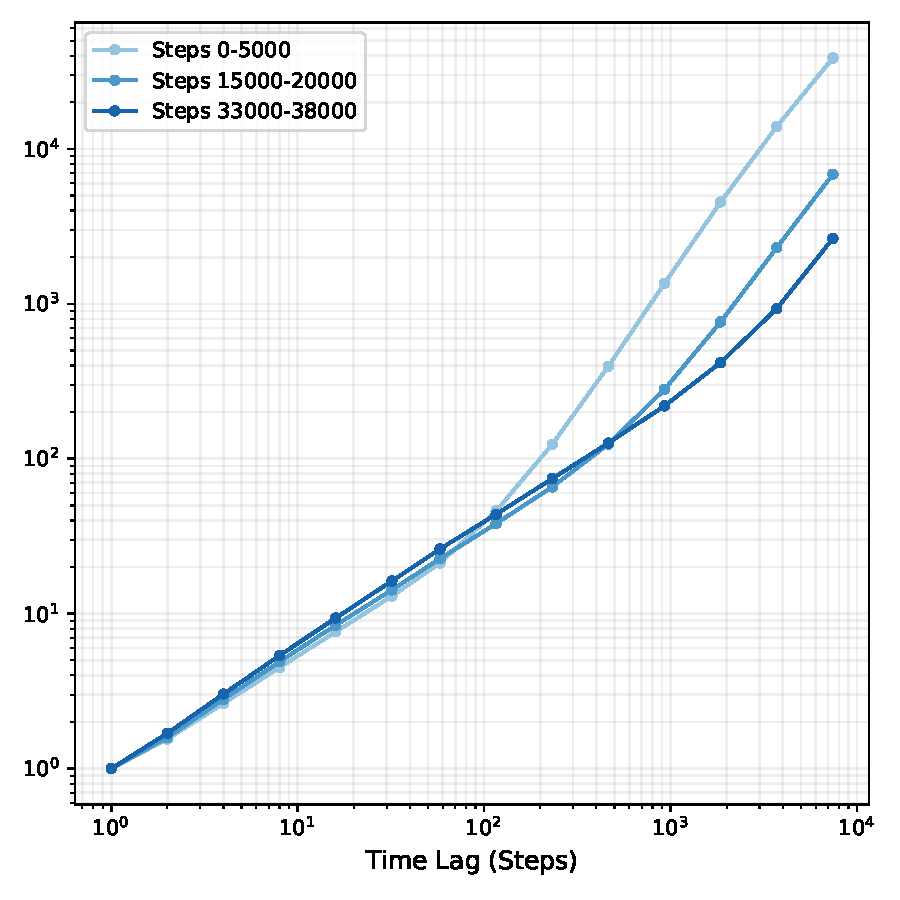
\includegraphics[width=\textwidth]{tamsd_evolution.pdf}
        \caption{Macro-scale kinetics ($\tau=58$)}
        \label{fig:tamsd_evo}
    \end{subfigure}
    \caption{Temporal evolution of $L_2$ weight displacement. (a) Step-wise dynamics ($\tau=1$) showing raw fluctuations and a 15-step rolling median. (b) Epoch-wise displacement ($\tau=58$) highlighting the contrast in trajectory smoothness between layers.}
    \label{fig:tamsd}
\end{figure}

The terminal hidden layer $W^9$ exhibits a remarkably consistent super-diffusive, near-ballistic regime across the entire range of observed time lags. The profile appears as a linear power law with an estimated exponent of $\gamma \approx 1.99$ for $\tau < 8$ epochs, slightly moderating to $\gamma \approx 1.76$ for macroscopic lags ($\tau > 8$ epochs). This persistent linearity suggests that the terminal layers are in a continuously driven state, undergoing directed translations within the parameter manifold.

In contrast, the first hidden layer $W^1$ displays a characteristic dynamical crossover. For shorter time lags ($\tau < 300$ steps), the shallow slope ($\gamma \approx 0.77$) is evidence of a sub-diffusive regime, where weights are likely constrained within local basins. However, as the time lag increases beyond a few epochs, the dynamics transition to a super-diffusive state ($\gamma \approx 1.49$). 

This observation supports the hypothesis of a hierarchical decoupling. The terminal layers operate as a directed engine, maintaining ballistic trajectories that drive classification performance. Meanwhile, the early layers function as a diffusive reservoir; while they are dominated by local stochasticity on microscopic scales, the emergence of super-diffusion over larger time horizons indicates a underlying directional gradient that provides a global guide for the learning process.

\begin{figure}[htbp]
    \centering
    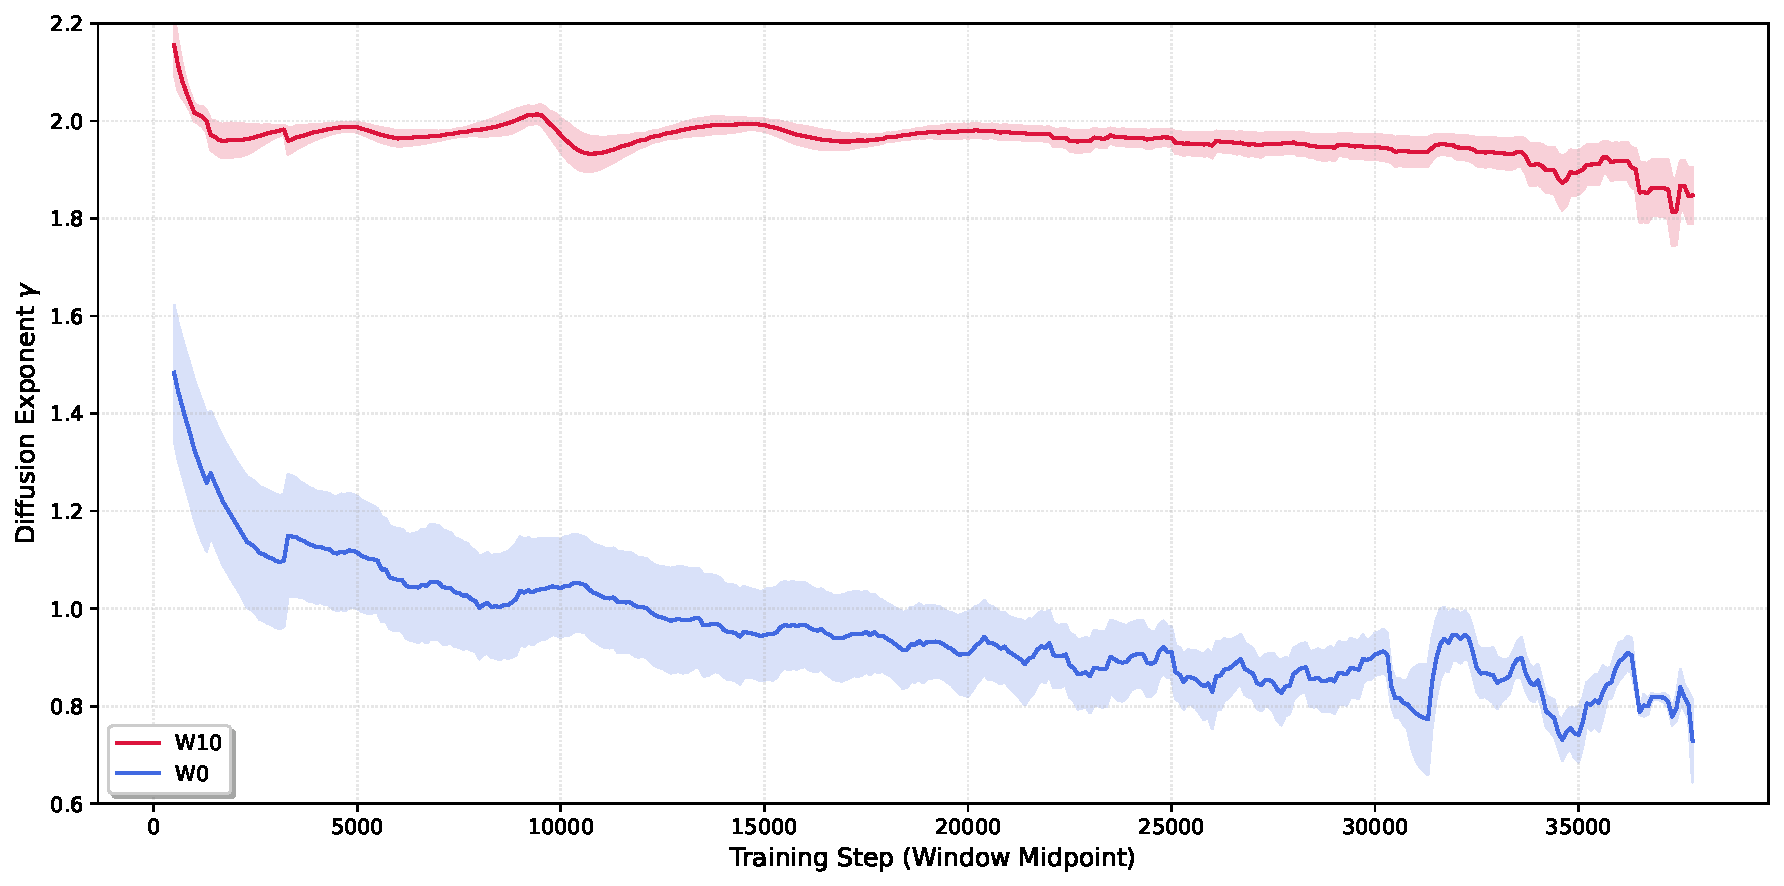
\includegraphics[width=0.8\textwidth]{diffusion_curve.pdf}
    \caption{Layer-wise correlation matrices of $L_2$ displacements ($\tau=1$). The emergence of distinct block-diagonal structures indicates a functional decoupling between the diffusive shallow layers and the ballistic terminal engine.}
    \label{fig:correlations}
\end{figure}
\section{Discussion}
\section{Conclusion}
\end{document}